\chapter{Communication in the swarm}

\paragraph*{}
This chapter gives the end results for the test from the Webots simulation on the sub-task \textbf{Communication in the swarm}. This sub-task resolves around the assumption that the \textit{swarm fleet is capable of object detection}, which is the key for task parallelization in our system. The main components of the communication system consist of the protocol, the robot's modes (states), consensus, and system integration.

\paragraph*{}
In general, the main robot we use is the Burger model of the third version of the TurtleBot robot, which has two functioning motors and a pre-built LiDAR system. Additionally, three more basic nodes are added to the TurtleBot object, which are the following: Firstly, the GPS node (Figure 2.1), this module is installed to obtain the robot’s position in the simulated world. This direct approach is used because the localization and mapping process is not available yet. Secondly, the Emitter node (Figure 2.2), this module is added to the robot to model a broadcast behavior. Thirdly, the receiver node (Figure 2.3), this module is connected as an accompaniment to the Emitter Class because the emitter node does not support both emitting and receiving functionalities. By combining all the devices, the basic simulation of swarm robotics communication is completed.

\begin{figure}[!htb]
    \minipage{0.32\textwidth}
        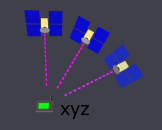
\includegraphics[width=\linewidth]{assets/images/communication/devices/gps.png}
        \caption{GPS node}\label{fig:GPS}
    \endminipage\hfill
    \minipage{0.32\textwidth}
        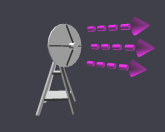
\includegraphics[width=\linewidth]{assets/images/communication/devices/emitter.png}
        \caption{Emitter node}\label{fig:Emitter}
    \endminipage\hfill
    \minipage{0.32\textwidth}%
        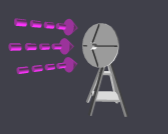
\includegraphics[width=\linewidth]{assets/images/communication/devices/receiver.png}
        \caption{Receiver node}\label{fig:Receiver}
    \endminipage
\end{figure}

This approach allows simple communication in the swarm system and awareness of other robot members in the swarm system. We then further build the system's protocol to ensure useful and safe information is transmitted across a reliable platform. These messages are processed through states combining structured communication with dynamic state transitions. 

\paragraph*{}
The protocol is built to support the incoming series of structured messages in a queue (Table 2.1) and robot states (Table 2.2).

Messages such as [probe] is used for updating position data. When an object is detected, a [task] message is broadcast, designating the detecting robot as the task master and informing the object's location to others. If conflicts occur, with two or more robots detecting the object at the same time, the robots will send a [task\_conflict] message, notifying other robots, and resolve them through a priority-based reassignment. Once tasks are completed, the [task\_successful] message signals the robot to transition to the next stage.

\begin{table}[ht]
\centering
\begin{tabular}{|p{3cm}|p{12cm}|}
\hline
 probe & Broadcasts real-time position data for efficient task coordination. 
 \newline \textbf{Sender}: Sends robot's position data. 
 \newline \textbf{Receiver}: Updates information the robot\_entries dictionary. 
 \newline \textbf{Format}: \{[probe], robot\_id, message\_id, (robot\_position["x"], robot\_position["y"], robot\_position["theta"])\} \\ 
 \hline
 object\_detected & Broadcasts the encounter of the target object. 
 \newline \textbf{Sender}: Sends object's position data. \newline \textbf{Receiver}: Changes its state to \textit{idle} and waits for further action. \newline \textbf{Format}: \{[object\_detected], robot\_id, found cylinder @ \{cylinder\_position\}\} \\ 
 \hline
 task & Broadcasts the assigning of a new taskmaster for the path planning. 
 \newline \textbf{Sender}: Sends an initiative to assign itself as the taskmaster. 
 \newline \textbf{Receiver}: Changes its state to \textit{task} and report conflicting status. 
 \newline \textbf{Format}: \{[task], robot\_id, message\_id, cylinder\_position\}\\ 
 \hline
 task\_conflict & Broadcasts the conflict occurs in task master assignment. 
 \newline \textbf{Sender}: Sends conflict information to other robots. \newline \textbf{Receiver}: Change its state to \textit{reassign}. 
 \newline \textbf{Format}: \{[task\_conflict], robot\_id, message\_id, priority\_queue\}\\ 
 \hline
 task\_successful & Broadcasts a success operation in task master assignment.  
 \newline \textbf{Sender}: Confirms the success of the operation and the task master. 
 \newline \textbf{Receiver}: Ensures all data and information complies to itself.
 \newline \textbf{Format}: \{[task\_successful], robot\_id, message\_id, task\_master\}\\ 
 \hline
 path\_following & Broadcasts a notification for robots to follow the given paths.  
 \newline \textbf{Sender}: Sends planned path to each robots. 
 \newline \textbf{Receiver}: Changes its state to \textit{path\_following}, and updates its path.
 \newline \textbf{Format}: \{[path\_following], robot\_id, message\_id, paths\_json\}\\ 
 \hline
\end{tabular}
\caption{Message Types}
\end{table}

\newpage

Each message may trigger a state transition; this is done by the communicator handling the message from the queue. Robots may start in the \textit{idle} or \textit{NaN} state, finding the object. If one of the robots detects an object, it will change to \textit{consensus} state, where the task master is selected and agreed upon in this phase. The taskmaster then transitions to \textit{path\_finding} to generate navigation routes for both itself and other robots. After that, when all robots receive their own routes to the destination, it will switch to the \textit{path\_following} stage.

\begin{table}[ht]
\centering
\begin{tabular}{|p{3cm}|p{12cm}|}
\hline
 idle (Default) & State where the robot halt and wait for instructions\\ \hline
 consensus & State where an agreement of the task master is decided.\\ \hline
 path\_finding & State where the task master generates navigation paths for all robots.\\ \hline
 path\_following &  State where the robot follows it's path.\\ \hline
 task & States that handles task management, particularly conflicts.\\ \hline
 reassign & States that reassigns the task master when conflicts arise.\\ \hline
\end{tabular}
\caption{Robot States}
\end{table}

The consensus mechanism used in this project is inspired by the Paxos Algorithm but is more lightweight. We are making a protocol that allows a group of robot agents to agree on a single value, even if some of the agents fail to be responsive. In our case, the major concern that we need to tackle is a scenario of multiple robots detecting the object at the same time, and the allocation of taskmasters needs to be agreed upon by all parties. To do that, we added an intermediate state after an object is detected. And if the detected robot receives \textit{object\_detection} from other robots before receiving confirmation messages, it will raise the error and can send \textit{task\_conflict} to other robots.

\begin{figure}[!htb]
    \minipage{0.5\textwidth}
        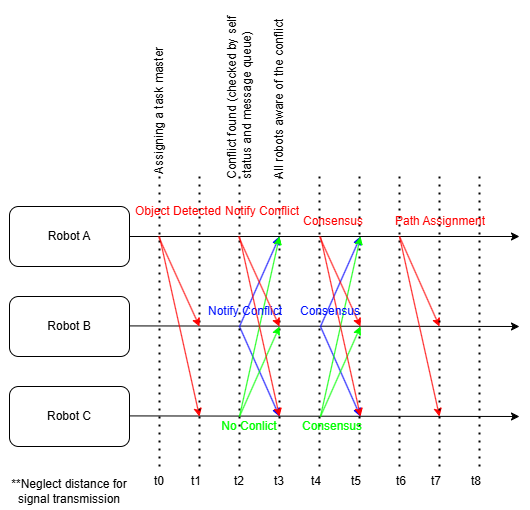
\includegraphics[width=\linewidth]{assets/images/communication/outputs/consensus_conflict.png}
        \caption{Conflict State}\label{fig:GPS}
    \endminipage\hfill
    \minipage{0.5\textwidth}
        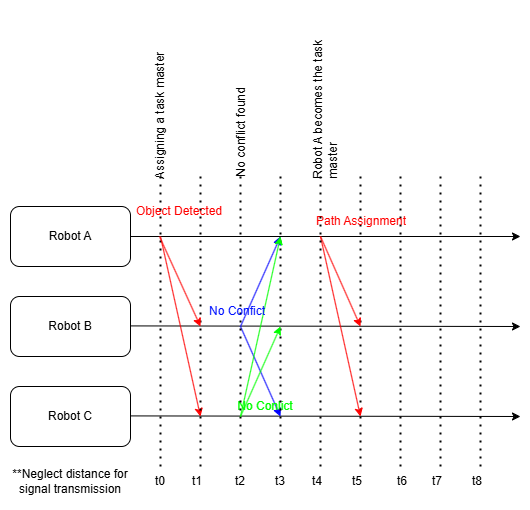
\includegraphics[width=\linewidth]{assets/images/communication/outputs/consensus_normal.png}
        \caption{Normal State}\label{fig:Emitter}
    \endminipage\hfill
\end{figure}
